\section{Исследовательский раздел \hfill}
\vspace{\baselineskip}

В данном разделе будет приведена демонстрация работы программы, а также произведен сравнительный анализ алгоритмов на основе времени их работы и затрачиваемой памяти.

\subsection{Технические характеристики}

Технические характеристики устройства, на котором выполнялось тестирование:

\begin{itemize}
	\item операционная система Windows 10.
	\item память 8 ГБ.
	\item процессор Intel® Core™ i5-6260U @ 1.80ГГц.
\end{itemize}

Замеры времени выполнения реализаций алгоритмов проводились на ноутбуке, включенном в сеть электропитания. Во время тестирования ноутбук был нагружен только встроенными приложениями окружения, а также непосредственно разработанным приложением.

\subsection{Демонстрация работы программы}

На рисунке \ref{fig:program-output} представлен пример работы программы. Пользователь вводит две строки, в результате работы программы на экран выводятся искомые расстояния и матрицы расстояний для всех случаев, кроме рекурсивного без кеша.
\clearpage

\begin{figure}[h!btp]
	\centering
	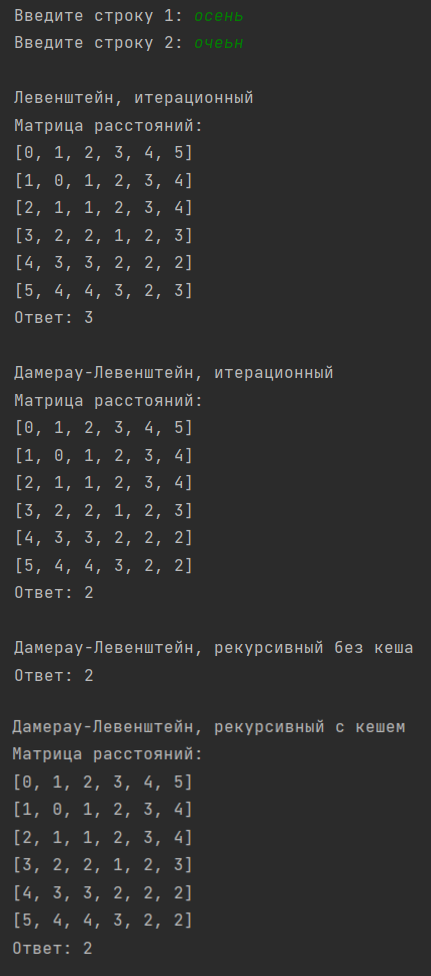
\includegraphics[width=240pt]{inc/program-output.png}
	\caption{Пример работы программы}
	\label{fig:program-output}	
\end{figure}
\clearpage

\subsection{Сравнение времени выполнения реализаций алгоритмов}

Сравнение времени выполнения реализаций алгоритмов производилось на строках длиной от 0 до 10 с шагом 1 для всех реализаций и на строках длиной от 0 до 200 с шагом 10 для реализаций, использующих матрицы расстояний.

Так как замеры времени имеют некоторую погрешность, они производились 20 раз для каждой реализации алгоритма и длины строки, а затем вычислялось среднее время работы реализации с текущей длиной строки. 
 
На рисунке \ref{fig:time_all} приведены результаты сравнения времени работы всех реализаций в секундах. Как видно на графике, реализации, использующие матрицы расстояний, работают значительно быстрее рекурсивной реализации без кеширования. Это обусловлено отсутвием в первых вызова функций для вычисления значений, которые уже были подсчитаны ранее.
\clearpage

\begin{figure}[h!btp]
	\centering
	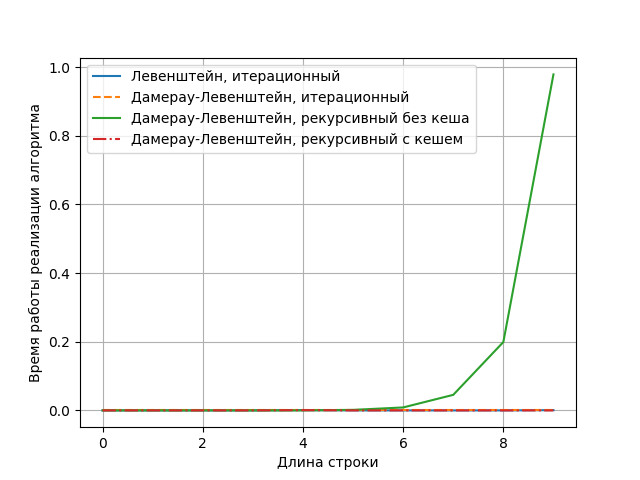
\includegraphics[width=400pt]{inc/time_all.png}
	\caption{Сравнение времени работы реализаций алгоритмов}
	\label{fig:time_all}	
\end{figure}

Сравним отдельно реализации, использующие матрицы расстояний.
 
На рисунке \ref{fig:time_w_matr} приведено сравнение времени выполнения реализаций итерационного алгоритма поиска расстояния Левенштейна, итерационного и рекурсивного с кешированием алгоритмов поика расстояния Дамерау"=Левенштейна. Время их работы растет соизмеримо, что обусловлено их схожестью в отсутствии вызова функций для вычисления значений, которые уже были подсчитаны ранее. Однако рекурсивная реализация с кешированием все же работает дольше, так как в ней тратится время на рекурсивный вызов. 
\clearpage

 \begin{figure}[h!btp]
    \captionsetup{justification=centering}
	\centering
	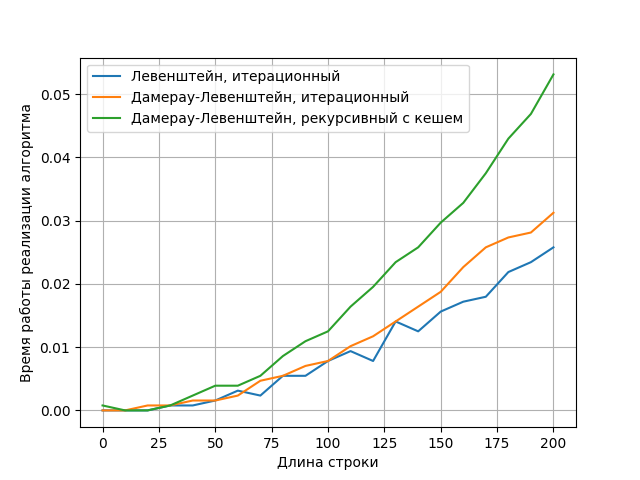
\includegraphics[width=400pt]{inc/time_w_matr.png}
	\caption{Сравнение времени работы реализациий алгоритмов, использующих матрицы растояний}
	\label{fig:time_w_matr}	
\end{figure}

\subsection{Оценка памяти}

Пусть $m$, $n$ - длины строк $S1$ и $S2$ соответственно. 

Затраты памяти для итеративного алгоритма поиска расстояния Левенштейна с матрицей расстояний:
	\begin{itemize}
		\item $2 \cdot sizeof(string\_pointer)$ (ссылки на строки $S1, S2$);
		\item $2 \cdot sizeof(int)$ (длины строк);
		\item $((m + 1) \cdot (n + 1)) \cdot sizeof(int)$ (матрица);
		\item $3 \cdot sizeof(int)$ (вспомогательные переменные).
	\end{itemize}
	Результат: $((m + 1) \cdot (n + 1) + 5) \cdot sizeof(int) + 2 \cdot sizeof(string\_pointer)$

Затраты памяти для итеративного алгоритма поиска расстояния Дамерау"=Левенштейна с матрицей расстояний:
	\begin{itemize}
		\item $2 \cdot sizeof(string\_pointer)$ (ссылки на строки $S1, S2$);
		\item $2 \cdot sizeof(int)$ (длины строк);
		\item $((m + 1) \cdot (n + 1)) \cdot sizeof(int)$ (матрица);
		\item $4 \cdot sizeof(int)$ (вспомогательные переменные).
	\end{itemize}
	Результат: $((m + 1) \cdot (n + 1) + 6) \cdot sizeof(int) + 2 \cdot sizeof(string\_pointer)$

Максимальная глубина стека вызовов при рекурсивной реализации равна сумме длин входящих строк. Ниже приведены оценки памяти для каждого вызова рекурсивной функции и итоговая затрачиваемая память с учетом максимальной глубины стека.

Затраты памяти для рекурсивного алгоритма поиска расстояния Дамерау"=Левенштейна (для каждого вызова):
	\begin{itemize}
		\item $2 \cdot sizeof(string\_pointer)$ (ссылки на строки $S1, S2$);
		\item $2 \cdot sizeof(int)$ (длины строк);
		\item $4 \cdot sizeof(int)$ (вспомогательные переменные).
	\end{itemize}
	Результат: $(m + n) \cdot (6 \cdot sizeof(int) + 2 \cdot sizeof(string\_pointer))$

Затраты памяти для рекурсивного алгоритма поиска расстояния Дамерау"=Левенштейна с использованием кеша (для каждого вызова): 
	\begin{itemize}
		\item $2 \cdot sizeof(string\_pointer)$ (ссылки на строки $S1, S2$);
		\item $2 \cdot sizeof(int)$ (длины строк);
		\item $((m + 1) \cdot (n + 1)) \cdot sizeof(int)$ (матрица).
	\end{itemize}
	Результат: $(m + n) \cdot (((m + 1) \cdot (n + 1) + 6) \cdot sizeof(int) + 2 \cdot sizeof(string\_pointer))$


\subsection{Вывод}
Рекурсивная реализация алгоритма поиска расстояния Дамерау-\newline Левенштейна без кеширования работает значительно дольше реализаций алгоритмов, в которых используется матрица расстояний.

Рекурсивный алгоритм с кешированием сравним с итерационными алгоритмами, однако его реализация все равно несколько дольше нерекурсивных аналогов.

Итерационные реализации алгоритмов Левенштейна и Дамерау-\newline Левенштейна сопоставимы по времени. Реализация алгоритма Дамерау-\newline Левенштейна незначительно дольше реализации Левенштейна, т.к. в первом случае имеет место дополнительная проверка на перестановку соседних символов.

По расходу памяти нерекурсивные алгоритмы проигрывают рекурсивному алгоритму без кеша на больших длинах строк: в первом случае максимальный размер используемой памяти растет пропорционально произведению длин строк, в то время как во втором -- пропорционально сумме длин строк.
